%!TEX root = ../../../report.tex
\section{Mechanics} % (fold)
\label{sec:mechanics}
This section deals with the mechanical design of the robot.
Based on the analysis performed in the chapter \ref{cha:analysis}, the mechancal design takes its results and carries out a specific analysis of each component.
Then, the conclusions are translated into a 3D model making a compromise between the requirements and manufacturability.

%!TEX root = ../../../../report.tex
\subsection{Pulleys and belts} % (fold)
\label{sub:pulleys_and_belts}
The section \ref{sec:joints} is dedicated to analyze and define what kind of motors and trasmision system is going to be used for each joint.
In the case of the knee and the ankle, the combination \textit{motor + gearbox + belt and pulleys} is chosen due to the preference of having the active actuator in the highest part of the link with the withdrawal of transfer the movement the the lowest.
This system has been design along with the torsional springs disussed in the section \ref{sub:compliance} where the rotation from the motor must feed the rotation of a serial rotational spring.
This implies the design of a system in which pulley and spring holder must be gathered.
The design of the pulley itself though, has been studied in terms of two factors: \textit{precision and backlash reduction} and \textit{integration with the serial rotational spring}.

\subsubsection{Precision and backlash reduction} % (fold)
\label{ssub:precision_and_backlash_reduction}
The goal of this design was to optimize the pulley to get a lack of backlash.
Despite the platform is going to be used mainly for self-learning controllers (e.g. based on neuronal networks) and then the mechanical optimization is not a priority, the reduction of mechanical uncertainty is always good.

After analyze all the current market several non-backlash solutions are found.
Stands out the Gates GT3 Synchronous Belts \footnote{http://www.gates.com/products/industrial/industrial-belts/synchronous-belts/powergrip-gt3-belts} that is assured to be suitable for the presented application.
The withdrawals of this design are the lack of time for ordering such parts and the increase in the final price of the product. 
However there is another important factor, the integration that must be done with the serial rotational spring.
% subsubsection precision_and_backlash_reduction (end)

\subsubsection{Integration with the serial rotational spring} % (fold)
\label{ssub:integration_with_the_serial_rotational}
Another solution is to design the pulley itself which would let to have a complete control of the design and manufacturability giving the possibility of integrate in a unique part design, the pulley for the transmission system and the spring holder.

At first, the GT3 design from Gates was intended to be designed.
However, its design is described in U.S. Patent Number 4,515,577, which doesn't allow its use.
Thus, the belts have been designed following the ISO 13050:2014 \cite{ISO13050} following the type T due to its focus in efficiency and reduction of backlash.
It is also appropriate for precision movements, high torques and low speeds, as our requirements.

The physical properties of the pulleys as the number of teeth, width, etc... have been chosen based on the ISO 5295:1987 \cite{ISO5295} and in sake of manufacturability.
As decided before, the pulley will belong to a part that will also have the task of holding the rotational serial spring.
This implies that the part will be designed to be 3D printed and thus, the criteria of design oriented to manufacturability must be applied.

Based on both ISO norms cited before and after some iterations based on experimental tests the pulley T2,5 of 19 teeth gave the expected behavior.
Both pulleys are the same so no reduction is given from the motor shaft to he other.
In the figure \ref{fig:motor_pulley}, a detail of the designed pulleys can be seen.
% subsubsection integration_with_the_serial_rotational (end)

% subsection pulleys_and_belts (end)
%!TEX root = ../../../../report.tex
\subsection{Gears} % (fold)
\label{sub:gears}

% subsection gears (end)
%!TEX root = ../../../../report.tex
\subsection{Impact force} % (fold)
\label{sub:impact_force}
In order to calculate the physical dimensions of some of the components, a bounding conditions have to be defined.
The presented case shows a peak of energy when landing after being jumped a estimated height.
This energy in then transmitted from the first contact point, the footprint, to the rest of the system, causing efforts that must be absorbed.
The components of the system must receive that energy under a controlled behavior -this is elastic deformations- assuring a longer life cycle of the legs.

Thus, some input parameters to calculate the impact force are assumed.
From this force will be sized all the consecutive components in the deformation chain.
Despite the deformation is of the whole system, the security coefficient assumed in here is going to be the calculation of all the components for that maximum force.

From the formula of the mechanical energy:
\begin{equation}
  E_{mechanical} = m g \Delta h + \frac{1}{2} m v^{2}
\end{equation}

The kinetic energy is negligible and only the energy form falling a certain height is supposed.
This energy is then translated into force by supposing a deformation of the whole body:
\begin{equation}
\label{eq:impact_force}
  F_{impact} = \frac{m g \Delta h}{t_{impact\_displacement}}
\end{equation}

The equation \ref{eq:impact_force} gives the force for sizing all the components.
Based on the input parameters defined in the appendix \ref{app:profile_selection} which are:
\begin{table}
\begin{center}
\begin{tabular}{c | c}
  Parameter & Value \\
  \hline
  Total mass [kg] & 1.5 \\
  Jumping height [m] & 0.1 \\
  Impact displacement [m] & 0.005
\end{tabular}
\caption{Input parameters for calculating the impact force}
\label{tab:input_parameter_impact_force}
\end{center}
\end{table}

The impact force is then:
\begin{equation}
  F_{impact} = \frac{m g \Delta h}{d_{impact\_displacement}} = 294.40 N 
\end{equation}
% subsection impact_force (end)
%!TEX root = ../../../../report.tex
\subsection{Limb profile} % (fold)
\label{sub:limb_profile}
Based on the requirements of weight and its distribution defined in the analysis of the joints \ref{sec:joints}, the links have been decided to have in the upper extreme the actuators. 
This leads to use a transmission system, such as belt and pulleys, which leaves for the rest of link a structural function that can also adopt the task of wiring placement.
Thus, a light weight section that satisfy the conditions of deformation and stress maximum will be chosen.
Carbon fiber is an ideal material to achieve this conditions of weight and stress so an quantitative analysis has been made calculating the optimal solution and then rounding it for all the possible profiles offered by the given provider.
The provider was chosen due to the previous experiences that the Mærsk Mc-Kinney Møller Institute had with carbon fiber orders.

The section profile offered \footnote{http://www.easycomposites.co.uk/\#!/cured-carbon-fibre-products/} are: \textit{Rod}, \textit{Tube}, \textit{Box}. The \textit{Stripe} and the \textit{Angle} are discarded due to its asymmetrical geometry that will will lead to less predictable scenarios.
The study case is show in the figure \ref{fig:impact_decomposition}, where the impact force can be decomposed in a pure bending effort and a pure compression.
Due to the resistance of the carbon fiber in pure compression is bigger than in bending, only this last case has been studied.
This studies should not completly follow the behaviour in real life due to the carbon fiber is not an isomorphic material.
However, the high security factor taken into account is expected to overcome this assumption.

\begin{figure}[ht!]
  \centering
  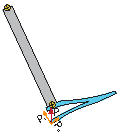
\includegraphics[width=.3\textwidth]{figures/impact_decomposition.pdf}
  \caption{Impact force decomposed}
  \label{fig:impact_decomposition}
\end{figure}

\subsubsection{Profile study} % (fold)
\label{ssub:profile_study}
  The bending effort causes two sort of problems: (1) the possible break in the supporting point and (2) the deformation suffered by the beam.
  The break will occur when the tensions created will be over the ultimate tension in compression or tension of the selected material.
  This comes defined in the equation \ref{eq:tension} for symmetric sections and when an only torque is being applied.
  \begin{equation}
  \label{eq:tension}
    \sigma _{compression} = \sigma _{tension} = \frac{M h_{CG}}{I_x}
  \end{equation}

  Meanwhile the deformation in the extreme can be calculated with the equation \ref{eq:deformation} if the case is simplified to the occurred in the figure \ref{fig:impact_decomposition}.
  This is, when the legs is completely stretched, what will cause the biggest stresses.

  \begin{figure}[ht!]
    \centering
    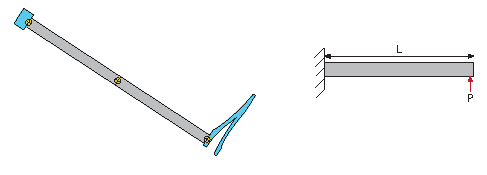
\includegraphics[width=\textwidth]{figures/bending_case.pdf}
    \caption{Simplified representation of the bending case}
    \label{fig:bending case}
  \end{figure}

  \begin{equation}
  \label{eq:deformation}
    y_L = \frac{P z^2}{6EI}(3L-z) = \frac{P L^2}{6EI}(2L) = \frac{P L^2}{3EI}
  \end{equation}


  For the selected profiles the equations that define the compression $\sigma _{compression}$ and tension efforts $\sigma _{tension}$, along with the deformation in the direcction of the applied force $y_L$ are shown, being:

  \begin{enumerate}
    \item $h_{CG}$: height of the center of gravity of the semi-half section from the geometrical center of the section.

    \item $E$: Elastic module.
  \end{enumerate}


  \noindent\begin{minipage}{0.2\textwidth}% adapt widths of minipages to your needs
      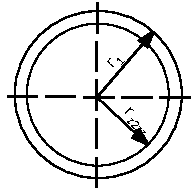
\includegraphics[width=\linewidth]{figures/profile_cylinder.pdf}
  \end{minipage}%
  \hfill%
  \begin{minipage}{0.8\textwidth}
    \begin{equation}
      \begin{aligned}
      \sigma _{compression} = \sigma _{tension} &= \frac{M h_{CG}}{I_x} = \frac{4 r_2}{\pi(r_2 ^4 - r_1 ^4)} M \\
      y_L &= \frac{P L^2}{3EI} = \frac{4 P L^2}{3 E \pi(r_2 ^4 - r_1 ^4)}\\
      h_{CG} &= r_2 \\
      I_x = I_y &= \frac{\pi}{4} (r_2 ^4 - r_1 ^4)
      \end{aligned}
    \end{equation}
  \end{minipage}

  \noindent\begin{minipage}{0.2\textwidth}% adapt widths of minipages to your needs
      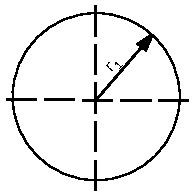
\includegraphics[width=\linewidth]{figures/profile_tube.pdf}
  \end{minipage}%
  \hfill%
  \begin{minipage}{0.8\textwidth}
    \begin{equation}
    \begin{aligned}
      \sigma _{compression} = \sigma _{tension} &= \frac{M h_{CG}}{I_x} = \frac{4}{\pi r_1 ^3} M\\
      y_L &= \frac{P L^2}{3EI} = \frac{4 P L^2}{3 E \pi r_1 ^4}\\
      h_{CG} &= r_1 \\
      I_x = I_y &= \frac{\pi r_1 ^4}{4}
      \end{aligned}
    \end{equation}
  \end{minipage}

  \noindent\begin{minipage}{0.2\textwidth}% adapt widths of minipages to your needs
      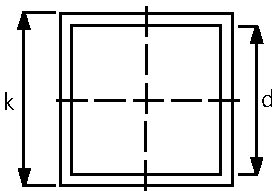
\includegraphics[width=\linewidth]{figures/profile_squared.pdf}
  \end{minipage}%
  \hfill%
  \begin{minipage}{0.8\textwidth}
    \begin{equation}
    \begin{aligned}
      \sigma _{compression} = \sigma _{tension} &= \frac{M h_{CG}}{I_x} = \frac{6 d}{(d^4 - k^4)}\\
      h_{CG} &= \frac{d}{2} \\
      y_L &= \frac{P L^2}{3EI} = \frac{4 P L^2}{E (d^4 - k^4)}\\
      I_x = I_y &= \frac{1}{12} (d^4 - k^4)
      \end{aligned}
    \end{equation}
  \end{minipage}
% subsubsection profile_study (end)

\subsubsection{Torque calculation} % (fold)
\label{ssub:torque_calculation}
  For both cases, the profile of the lower limb and the upper, the torque generated by the impact force determined in the section \ref{sub:impact_force}, is calculated.
  This torque is different in the lower and the upper limb due to the upper limb takes the distance from the foot to the hip while the other one is only from the foot to the knee:
  \begin{equation}
  \begin{aligned}
     M_{lower\ limb} = F \cdot d = 294.4 \cdot 0.2126 = 62.57 Nm\\
     M_{upper\ limb} = F \cdot d = 294.4 \cdot (0.2126 + 0.2622) = 139.73 Nm
  \end{aligned}
  \end{equation}
% subsubsection torque_calculation (end)

\subsubsection{Final limb parameters} % (fold)
\label{ssub:final_limb_parameters}
Following the criteria from the sections \ref{sec:dimensions} and \ref{sec:physical_properties} of size and materials, the presented formulas and the have been applied to all the profiles of the provider.
An iterative processes based on the outputs of the mathematical model \ref{cha:mathematical_model} has given a result the limb lengths shown in the table \ref{tab:limb_lengths}.

\begin{table}[ht!]
\centering
\caption{Final limb lengths}
\label{tab:limb_lengths}
\begin{tabular}{r|l}
  \textbf{Limb} & \textbf{Length [m]} \\ \hline
  Foot & 0.095 \\ \hline
  Lower limb & 0.212 \\ \hline
  Upper limb & 0.262    
\end{tabular}
\end{table}

\todo{Add hip and foot width with small explanation}

Then, the profiles have been analyzed calculating the torque from \ref{ssub:torque_calculation} and then applying the section \ref{ssub:profile_study} for each iteration.
The calculations of the last iteration are shown in the appendix \ref{app:profile_selection}.
These results have been then approved or discarded based on a \textit{maximum deformation} and \textit{ultimate tension} requirements, and are shown in the table \ref{tab:profile_selection}

\begin{table}[ht!]
\centering
\caption{Profile selection for each limb}
\label{tab:profile_selection}
\begin{tabular}{c|c|c}
  \textbf{Limb} & \textbf{Section} & \textbf{Dimensions} \\ \hline
  Lower limb & Tube & 20 mm and 1 mm thickness \\ \hline
  Upper limb & Tube & 20 mm and 1 mm thickness 
\end{tabular}
\end{table}

% subsubsection profile_selection (end)



% subsection limb_profile (end) 
%!TEX root = ../../../../report.tex

\subsection{Bearings} % (fold)
\label{sub:bearings}
In the section \ref{sub:impact_force} the force for sizing the bearings of the knee and the ankle was calculated.
The bearing elected would be such that allows dynamic loads of more than the impact force while keeping as small as possible to reduce the added weight to the robot.
On the other hand, the internal diameter comes defined by the rod diameter calculated in the section \ref{sub:rods}.

An estimation of nominal life of the bearing can be done from the Dynamic Load Rating (C), the Dynamic Equivalent Load (P) and the Life Rime Coefficient for a Ball Bearing (p) (being p=3 for balls bearings).
The equation \ref{eq:service_life_bearing}, shows the nominal life of a ball bearing that can be used in order to calculate the nominal life for a specific application.
It is also worth to mention that the Dynamic Equivalent Load (P) is divided by the number of bearings in which the force is spread.
\begin{equation}
  \label{eq:service_life_bearing}
  L_{10} = \frac{10^{6}}{60 n} \left(\frac{C}{P}\right)^{p}
\end{equation}

The term $L$ is the service life of a bearing (in number of hours or rpm), in normal conditions of speed and load, in which the bearing is working until fail by fatigue. 
Whilst $L_{10}$ is based in a stadistical model that is defined as the 90\% of the bearing of the same type will withstand those loads for a longer time.
% subsection bearings (end)
%!TEX root = ../../../../report.tex
\subsection{Rods} % (fold)
\label{sub:rods}
As explained in section \ref{sub:bearings}, was decided to have two bearings per link (which gives four per joint) and a rod going through them.
This rod is then also used, in the case of the knee and the ankle, as a support for the pulleys that transmit the power from the pulley to the next link.

Three mechanical efforts bound its design:
\begin{enumerate}
  \item \textbf{Shear strenth}: in the case of the shear produced when an impact occurs and the rod of one link moves in the opposite direcction than its relative in the consecutive link.
  \item \textbf{Resistance to beding}: due to the bending effort that the tension of the belt is constantly applying in the rod of the  knee and the ankle.
  \item \textbf{Torsion}: due to the pulley in the knee and the ankle. 
  This effort is negligible because zero-friction bearings are supposed.
\end{enumerate}

  \subsubsection{Shear analysis} % (fold)
  \label{ssub:shear_analysis}
  The maximum shear stress is found in the diameter of the cylinder (y=0) and is:
  
  \noindent\begin{minipage}{0.2\textwidth}% adapt widths of minipages to your needs
  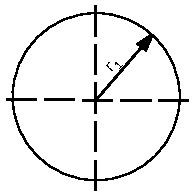
\includegraphics[width=\linewidth]{figures/profile_tube.pdf}
  \end{minipage}%
  \hfill%
  \begin{minipage}{0.8\textwidth}
    \begin{equation}
    \begin{aligned}
      \gamma_{yz} &= \frac{Q_y M_{x}^A*}{b(y) I_x} = \frac{Q}{r^2}\\
      M_{x}^{A_{y=0}} &= \frac{\pi r_1^2}{2} \\
      b(y=0) &= 2 r_1 \\
      I_x &= \frac{\pi r_1^4}{4}
      \end{aligned}
    \end{equation}
  \end{minipage}
  Given a tangent force Q, the shear stress can be calculated.
  If this is over the ultimate strength, the cylinder will break.
  % subsubsection shear_analysis (end)

  \subsubsection{Bending} % (fold)
  \label{ssub:bending}
  The beding analisys follows the one carried out in the section \ref{ssub:profile_study} for a cylinder.
  The equivalent force in this case is given by the tension of the belts, mainly the initial (thought there are other tensions that appear when the belts moves).
  Due to feasibility reasons an the lack of measurements units, some experimental tests trying differnt tensions and axis where carried out giving good results with a 3 mm rod or more.
  % subsubsection bending (end)

  \subsubsection{Sizing} % (fold)
  \label{ssub:sizing}
  The studies above have been tested for different diameters of rod starting from the smallest size given by the provider and increasing until both conditions are satisfied, due to the requirements of low weight.
  In case of using steel as material, the ultimate strength is supposed to be 250 MPa \footnote{https://en.wikipedia.org/wiki/A36\_steel}.
  And for the case of a rod of 3 mm of diameter, both stresses are under the restrictions.
  Thus, 3 mm rods are going to be used.
  % subsubsection sizing (end)
% section rods (end)
%!TEX root = ../../../../report.tex
\subsection{Spring integration} % (fold)

\todo{Springs selection (shortly)}

\label{sub:spring_integration}
In the section \ref{sub:compliance}, is justified the use of springs in order to walk and run efficiently. 
Later, an extensive analysis of the different possibilities to include compliance in the robot is done in the same section.
The figure \ref{fig:compliance_series} shows the analyzed configurations and their advantages and disadvantages are further discussed.
Due to the role that RuBi takes inside of the project, it is decided that all the configurations can be taken.
This is possible by making a system that allows to put elastic components in series and parallel that are easily replaceable.
Furthermore, a big range of springs have been ordered for the reasons in explained in \ref{sec_springs}.
All the springs can be placed due to the hole for inserting the springs has the diameter of the biggest one ordered plus an small clearance obtained from \ref{sub:arc_compensation}.

\subsubsection{SEA configuration} % (fold)
\label{ssub:sea_configuration}

In the section commented above, it is also determined the use of rotational springs for both series and parallel passive actuators.
This gives a more constrained design that is later used as a feature.
For example, in the section \ref{sub:pulleys_and_belts} is explained how the the pulley is integrated in a part that has the task of both being the place to put the spring and being the pulley.
The figure \ref{fig:serial_spring_pulley} shows this design.
This design shows the implementation of the SEA configurations that can be adjusted by changing the physical properties of the spring.
% subsubsection sea_configuration (end)

\subsubsection{PEA configuration} % (fold)
\label{ssub:pea_configuration}

% subsubsection pea_configuration (end)
The parallel spring is implemented by adding a spring directly attached to both parts of the joint.
The problem of the parallel passive actuators is the need of loading the spring for movements in which is maybe not appropriated.
As an example, the rest position of the parallel spring in the ankle could to be placed when the foot is at 90 degrees with its consecutive link, so the robot can be stood up without applying any extra torque in the motors to keep balance.
This would mean though to do an extra effort against the spring when taking off.

In the same line of giving all the possibilities to the user with the compliance, a system that allows to change the rest position of the parallel spring has been implemented.
This consists of one arm of the torsional spring attached to one of the links of the joint while the other arm can be fastened in different positions.
The figure \ref{fig:rotational_spring_rest_position} shows the transversal section of the part where the parallel spring can adopt different configurations. 
This gives the different PEA configurations by just changing the physical properties of the spring and by using an spring stiff enough in the SEA that would act as DD.

\begin{figure}[ht!]
	\centering
	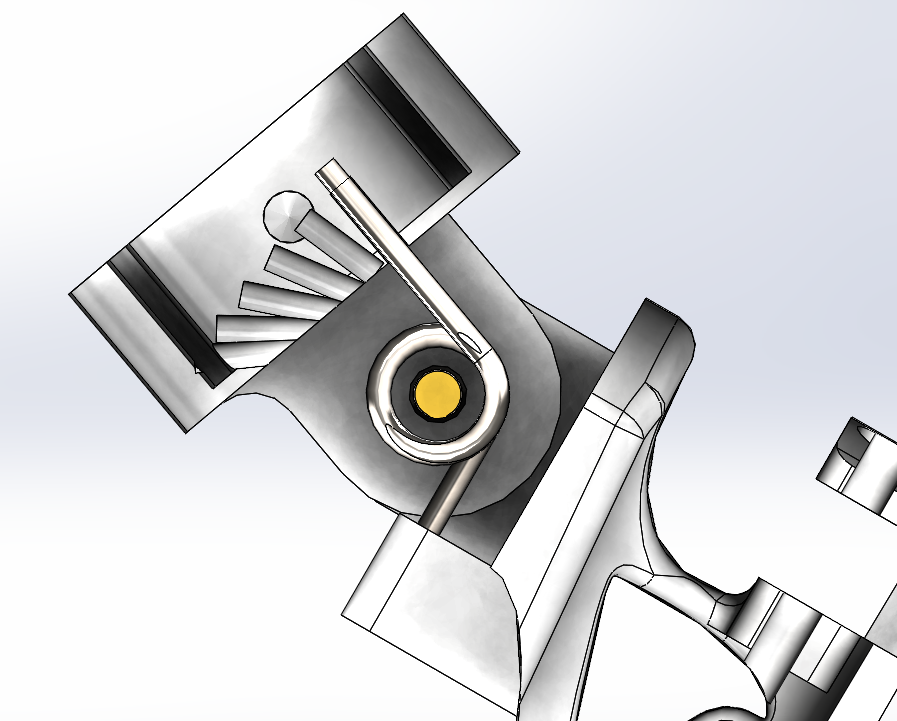
\includegraphics[width=0.75\textwidth]{figures/rotational_spring_rest_positions}
	\caption{Transversal section of the parallel spring resting positions in the left ankle.}
	\label{fig:rotational_spring_rest_position}
\end{figure}

\subsubsection{SEA + PEA configuration} % (fold)
\label{ssub:sea_pea_configuration}
The possibility of using both, SEA and PEA, configurations at the same time is given.
This lets the study of the combination of both configuration.
% subsubsection sea_pea_configuration (end)

\subsubsection{DD configuration } % (fold)
\label{ssub:dd_configuration}
Finally if no parallel spring is used and a spring stiff enough that doesn't add compliance to the system is placed, a DD configuration is achieved.
% subsubsection dd_configuration (end)

% subsection spring_integration (end)
%!TEX root = ../../../../report.tex

\subsection{Finite Element Method (FEM)} % (fold)
\label{sub:finite_element_method}

% subsection finite_element_method (end)
%!TEX root = ../../../../report.tex
\subsection{Computer-Aided Design (CAD)} % (fold)
\label{sub:computer_aided_design}

\begin{figure}[ht!]
    \centering
    \begin{subfigure}[b]{0.49\textwidth}
        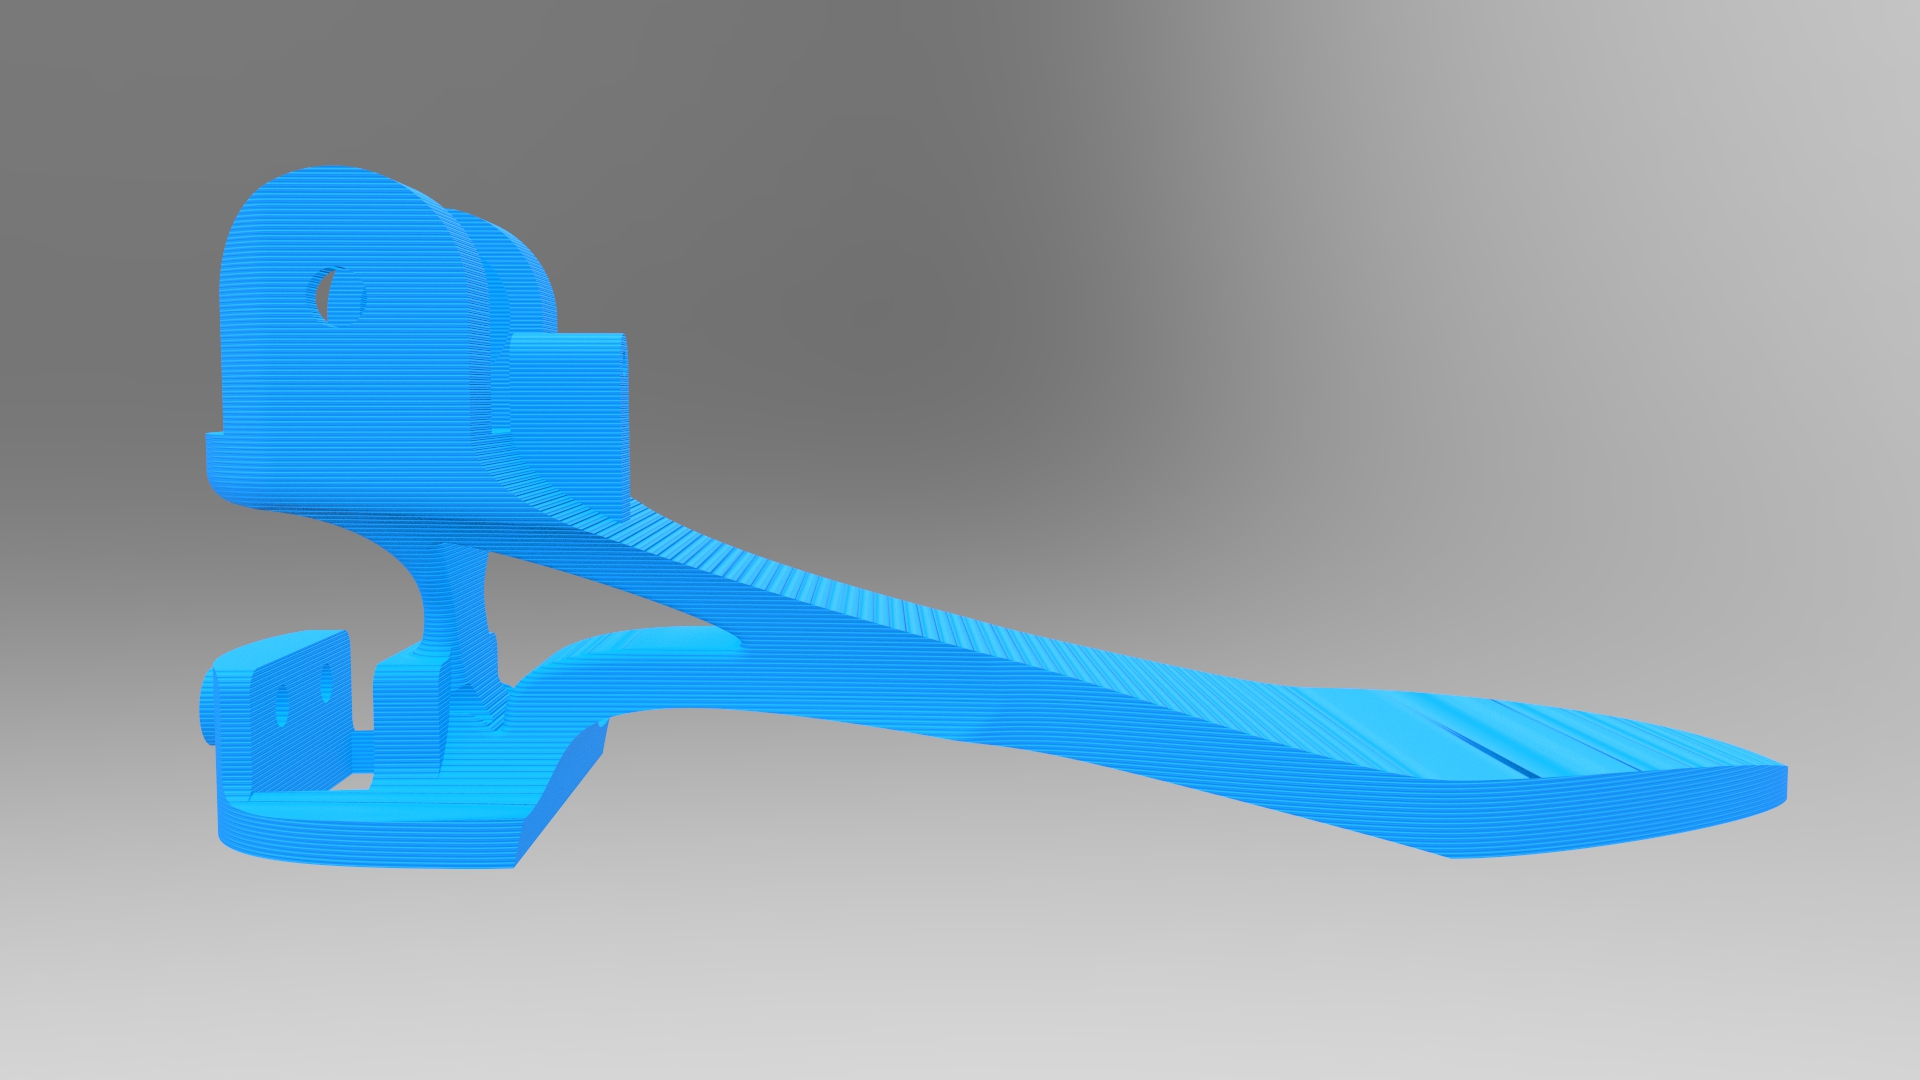
\includegraphics[width=\textwidth]{figures/legs_foot.jpg}
        \caption{Left foot}
        \label{fig:left_foot}
    \end{subfigure}
    \begin{subfigure}[b]{0.49\textwidth}
        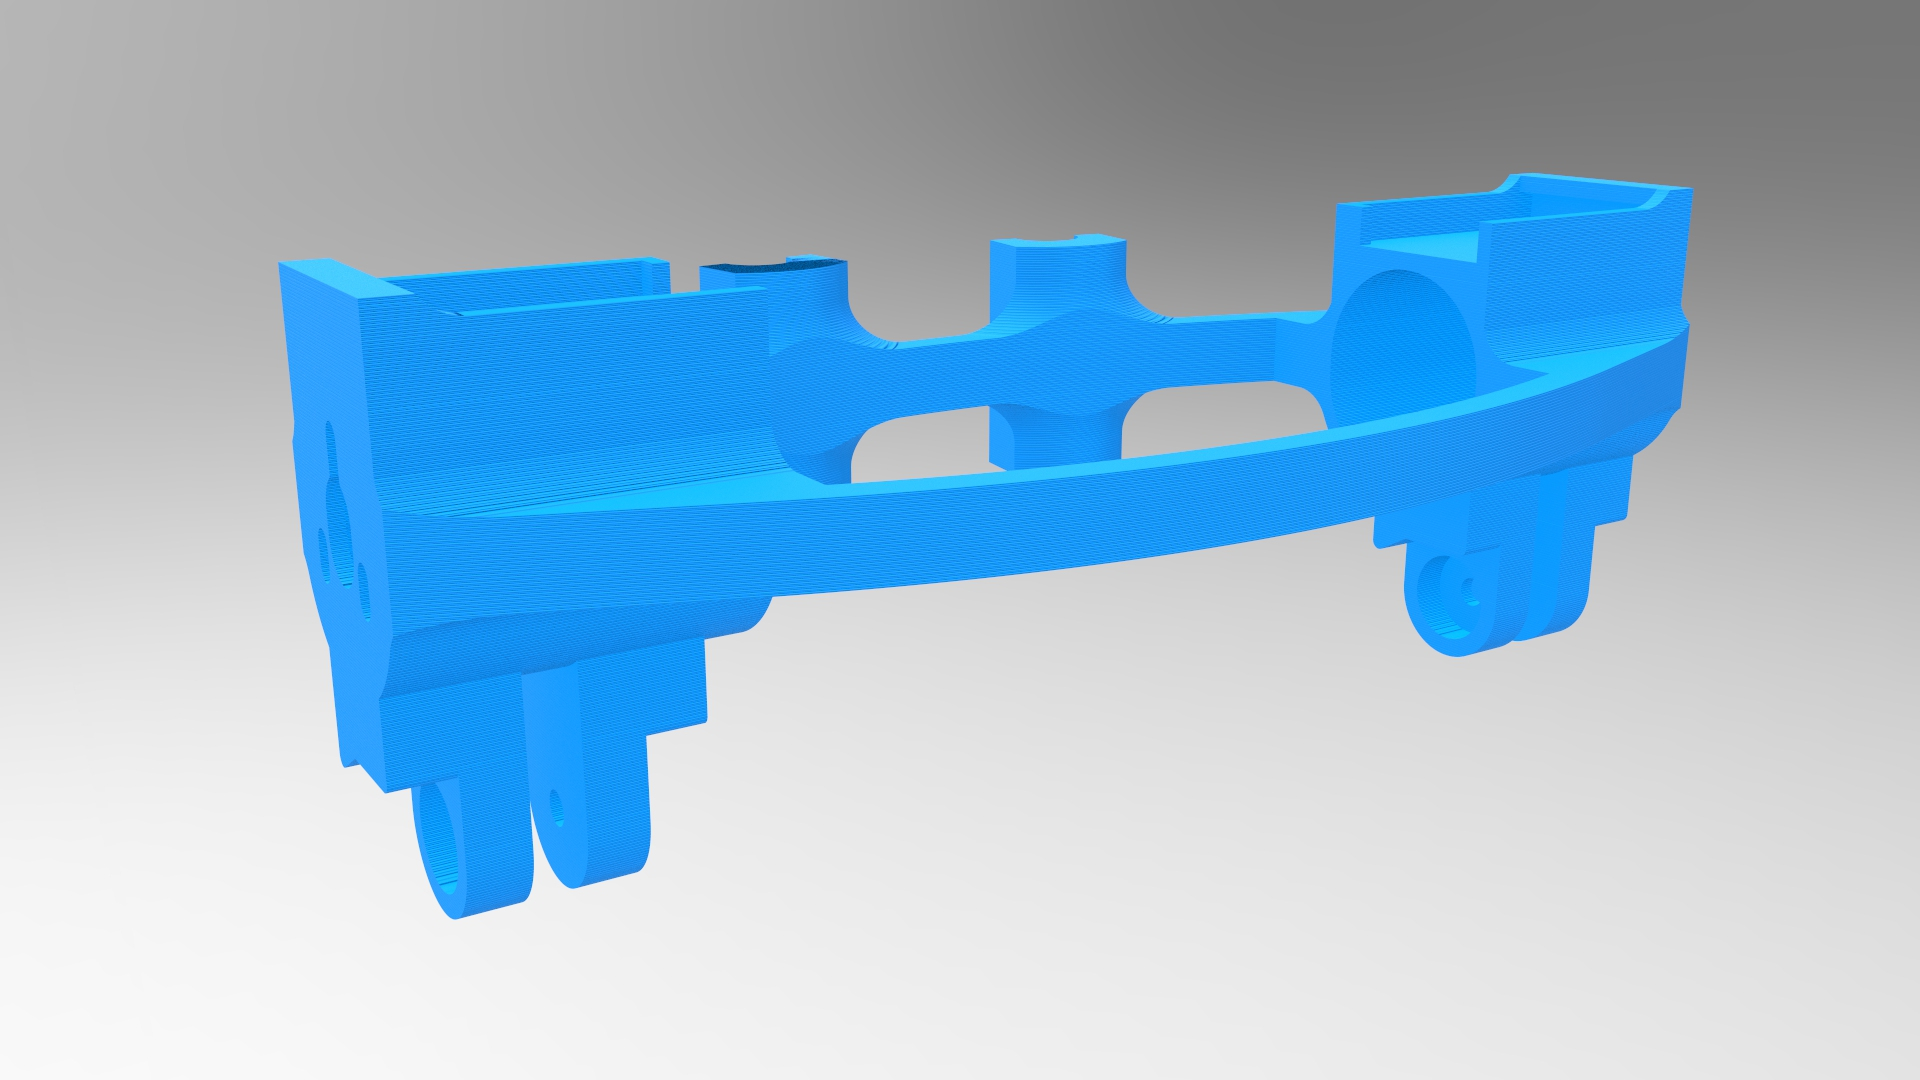
\includegraphics[width=\textwidth]{figures/legs_hip.jpg}
        \caption{Hip}
        \label{fig:hip}
    \end{subfigure}

    \begin{subfigure}[b]{0.49\textwidth}
        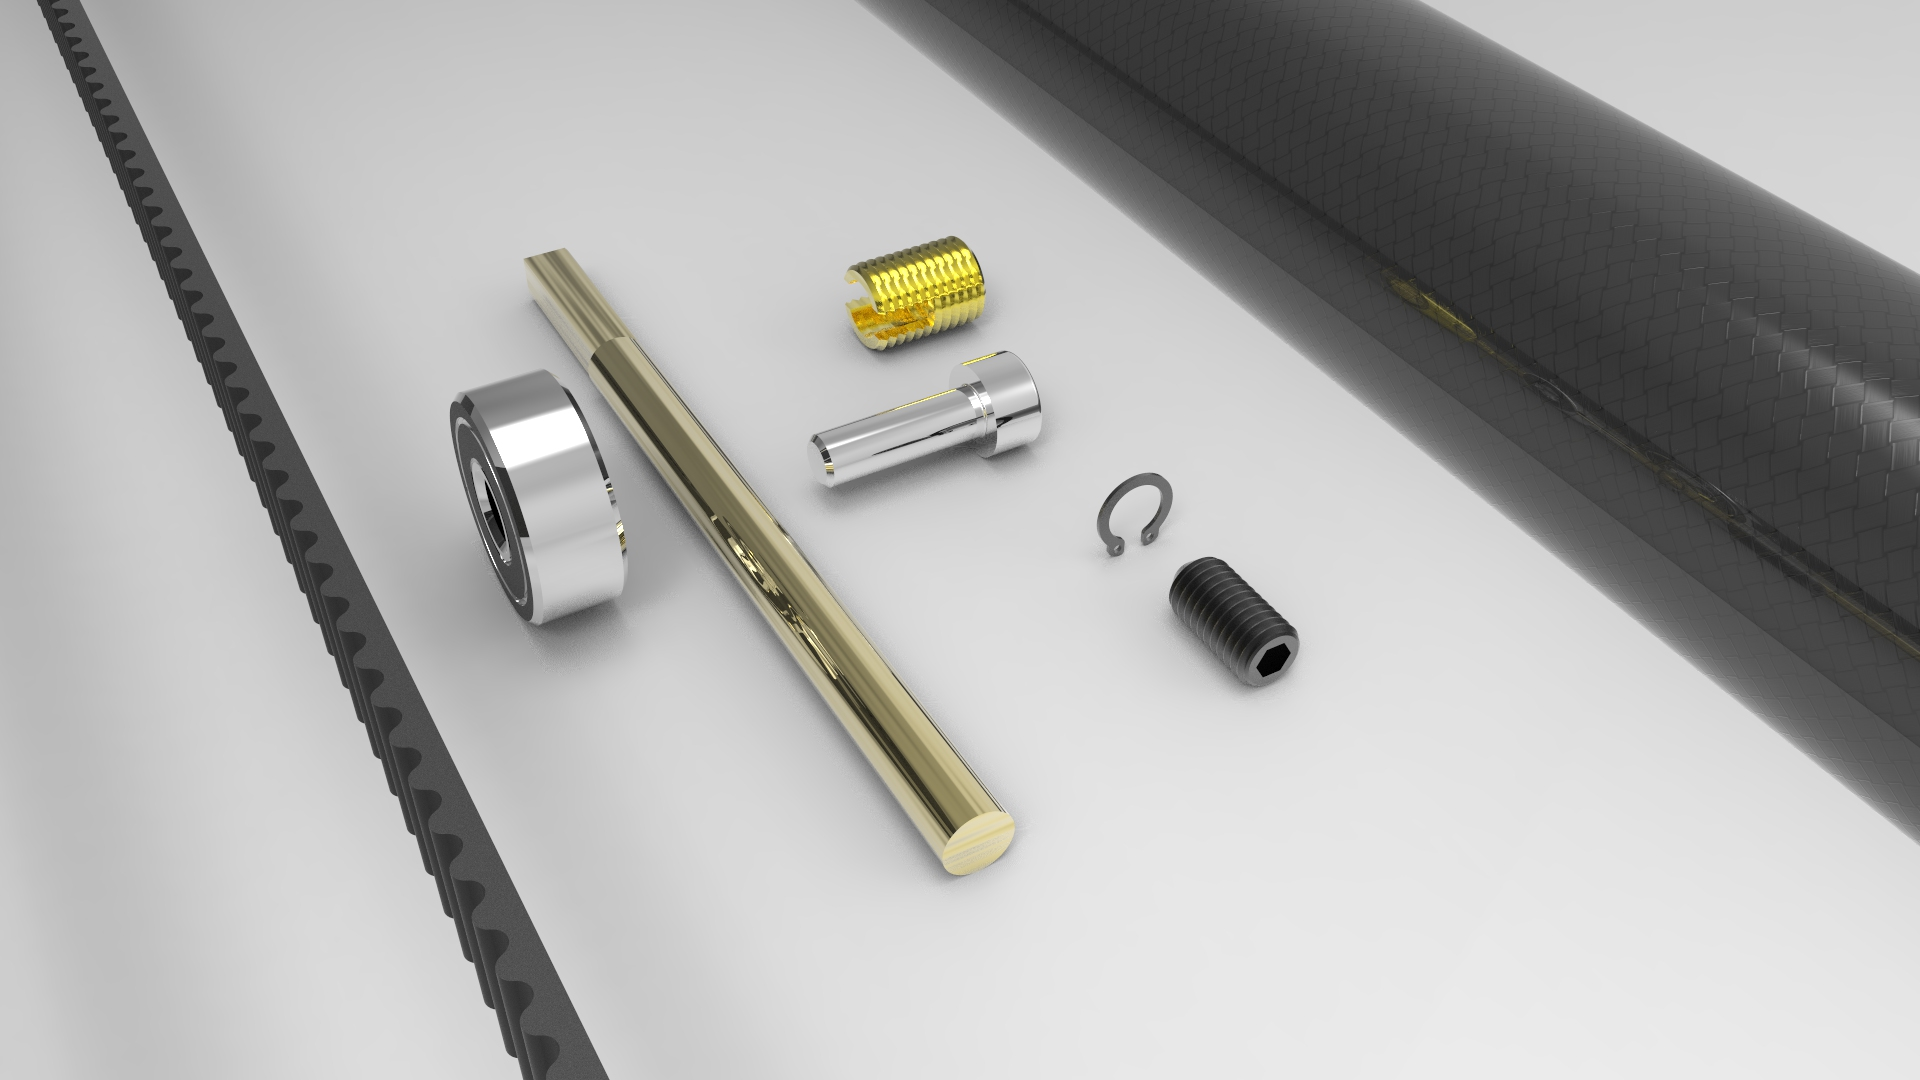
\includegraphics[width=\textwidth]{figures/legs_parts.jpg}
        \caption{Additional designed parts}
        \label{fig:mouse}
    \end{subfigure}
    \begin{subfigure}[b]{0.49\textwidth}
        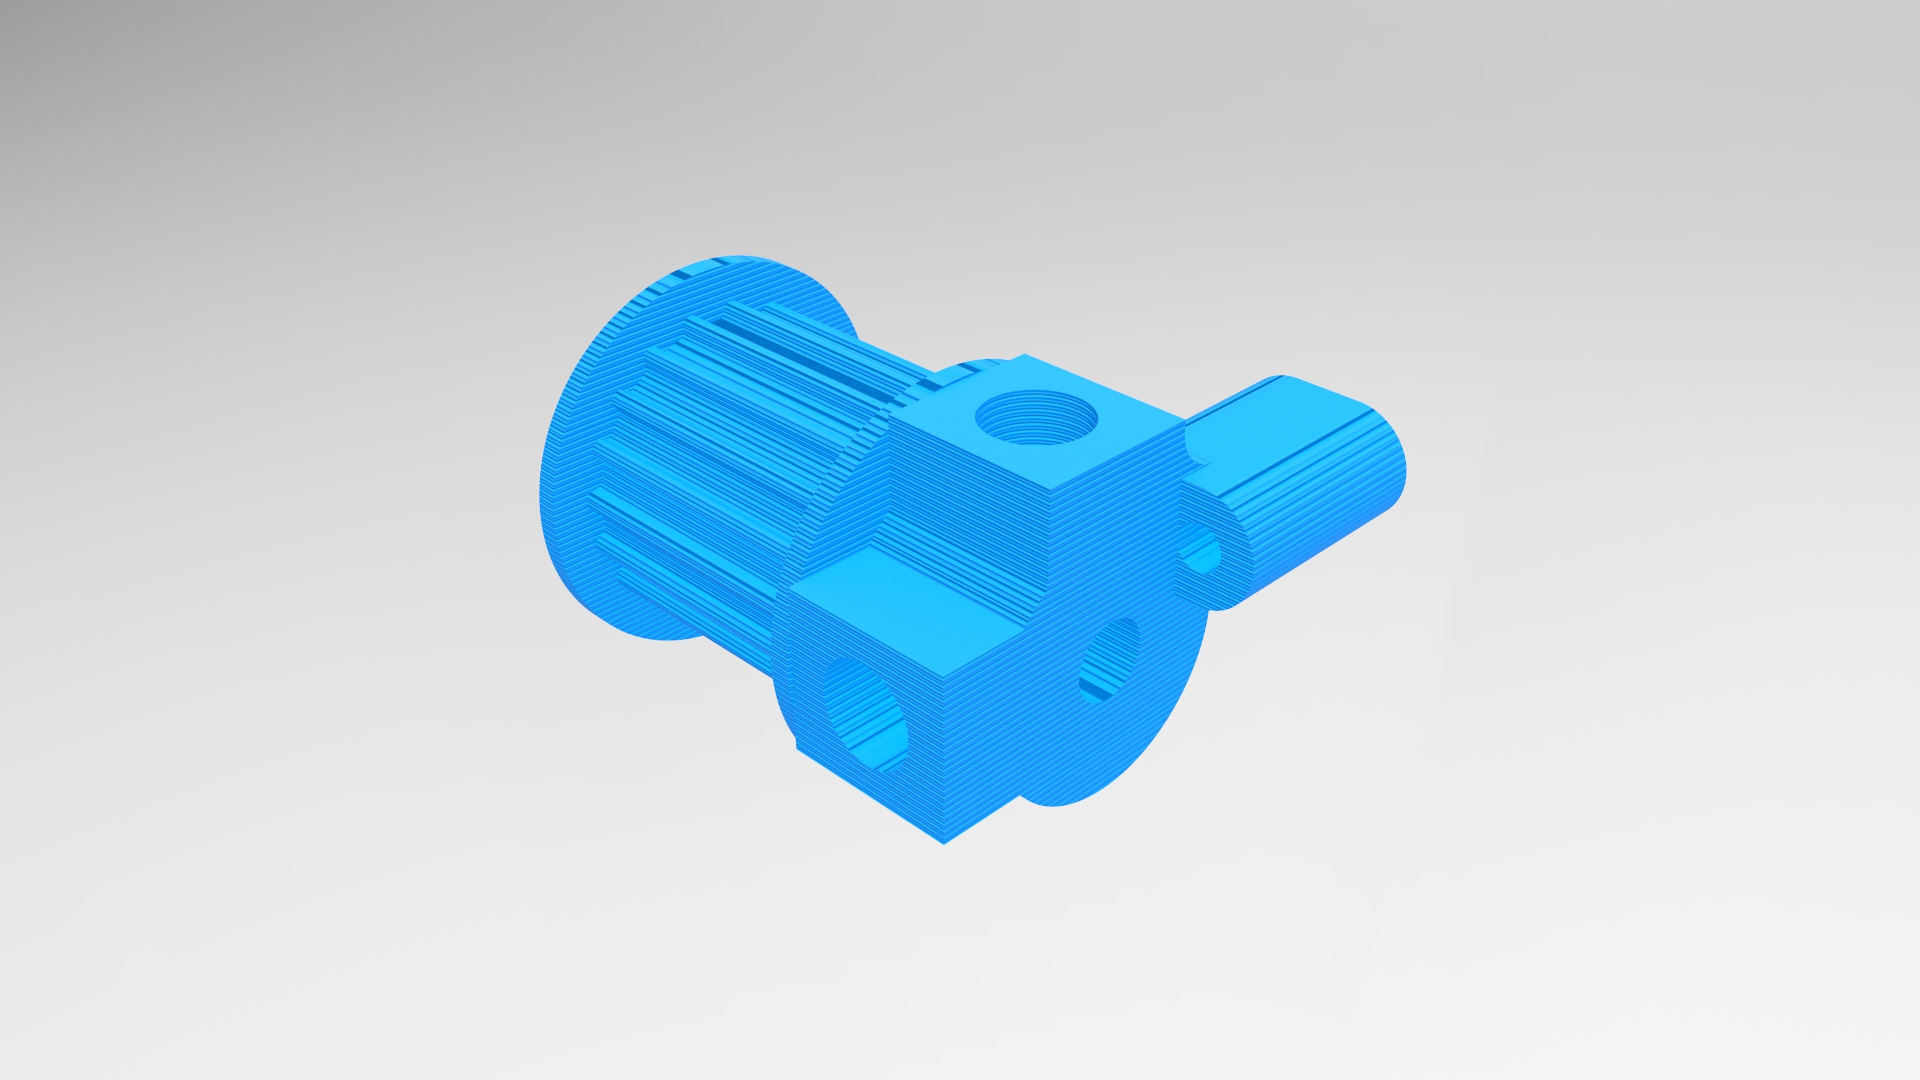
\includegraphics[width=\textwidth]{figures/legs_pulley.jpg}
        \caption{Left ankle serial spring pulley}
        \label{fig:serial_spring_pulley}
    \end{subfigure}

    \begin{subfigure}[b]{0.49\textwidth}
        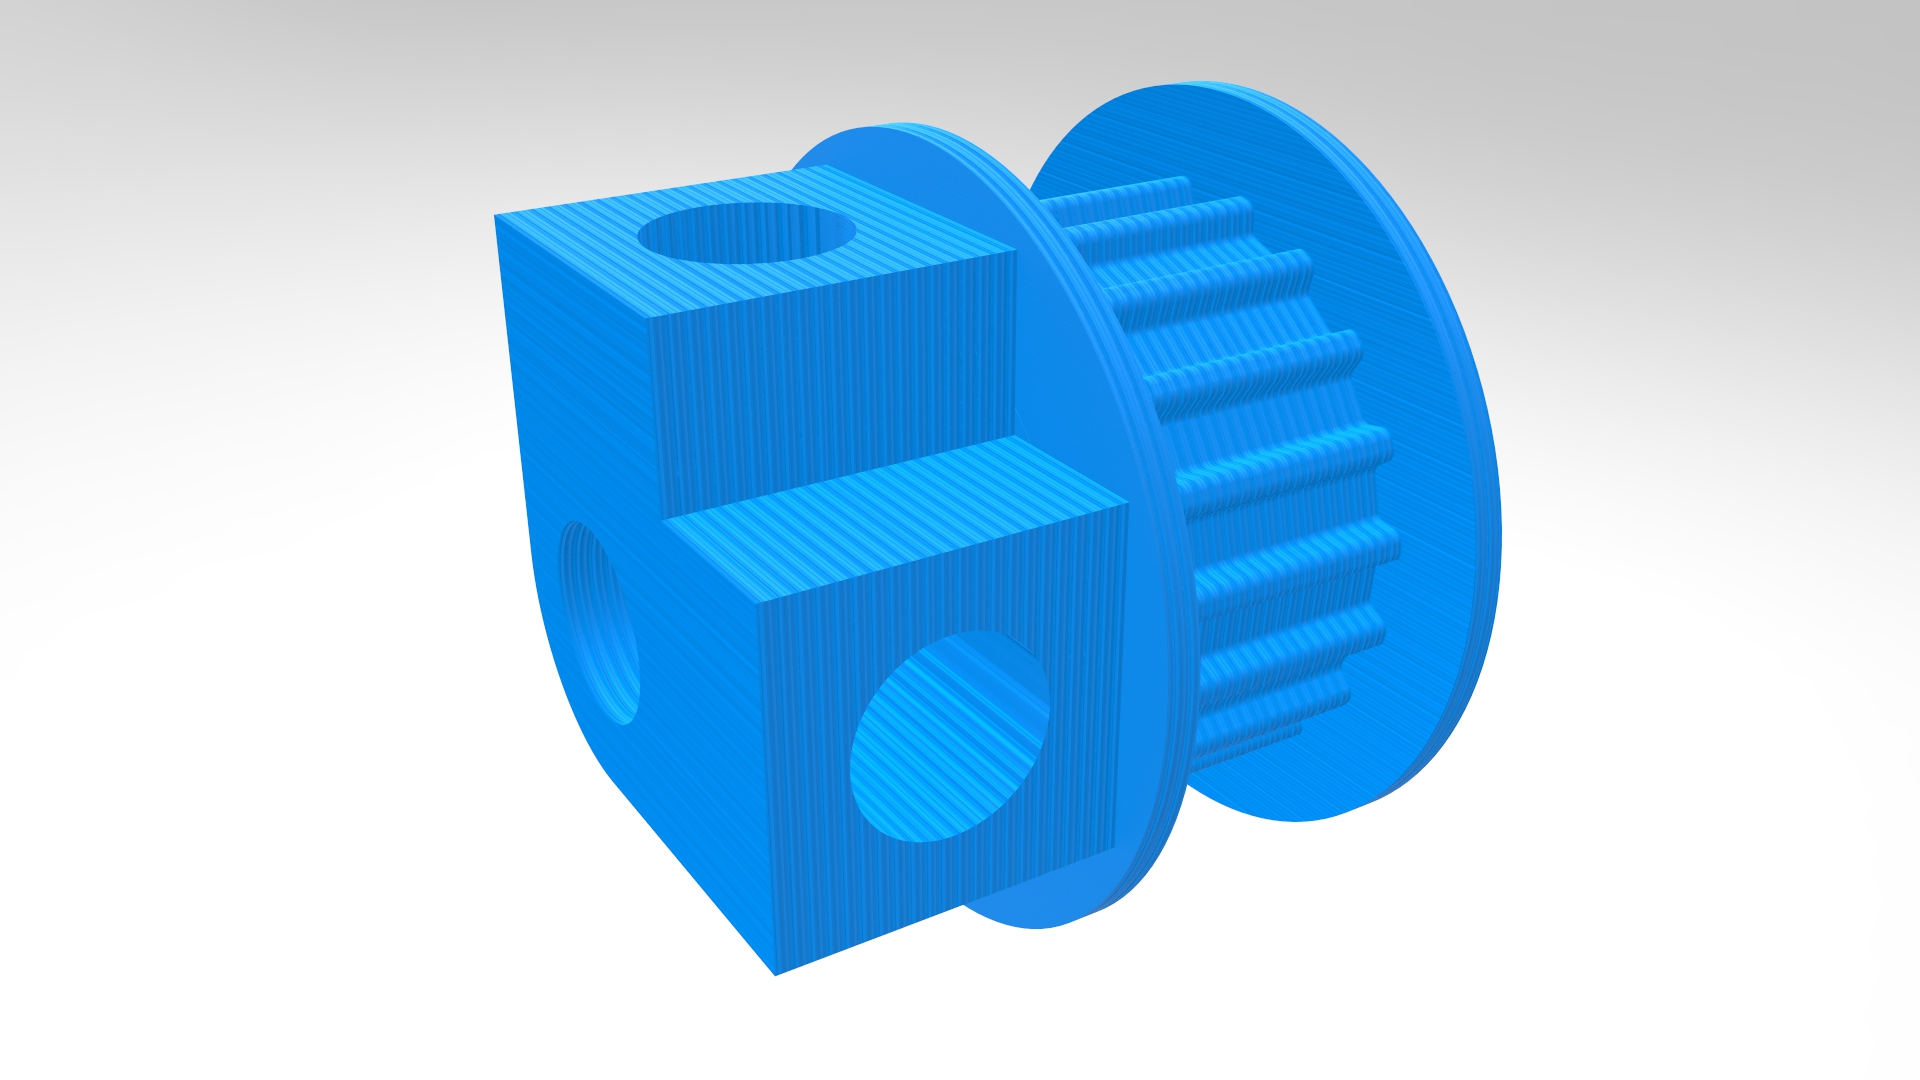
\includegraphics[width=\textwidth]{figures/legs_pulley_motor.jpg}
        \caption{Motor pulley}
        \label{fig:motor_pulley}
    \end{subfigure}
    \begin{subfigure}[b]{0.49\textwidth}
        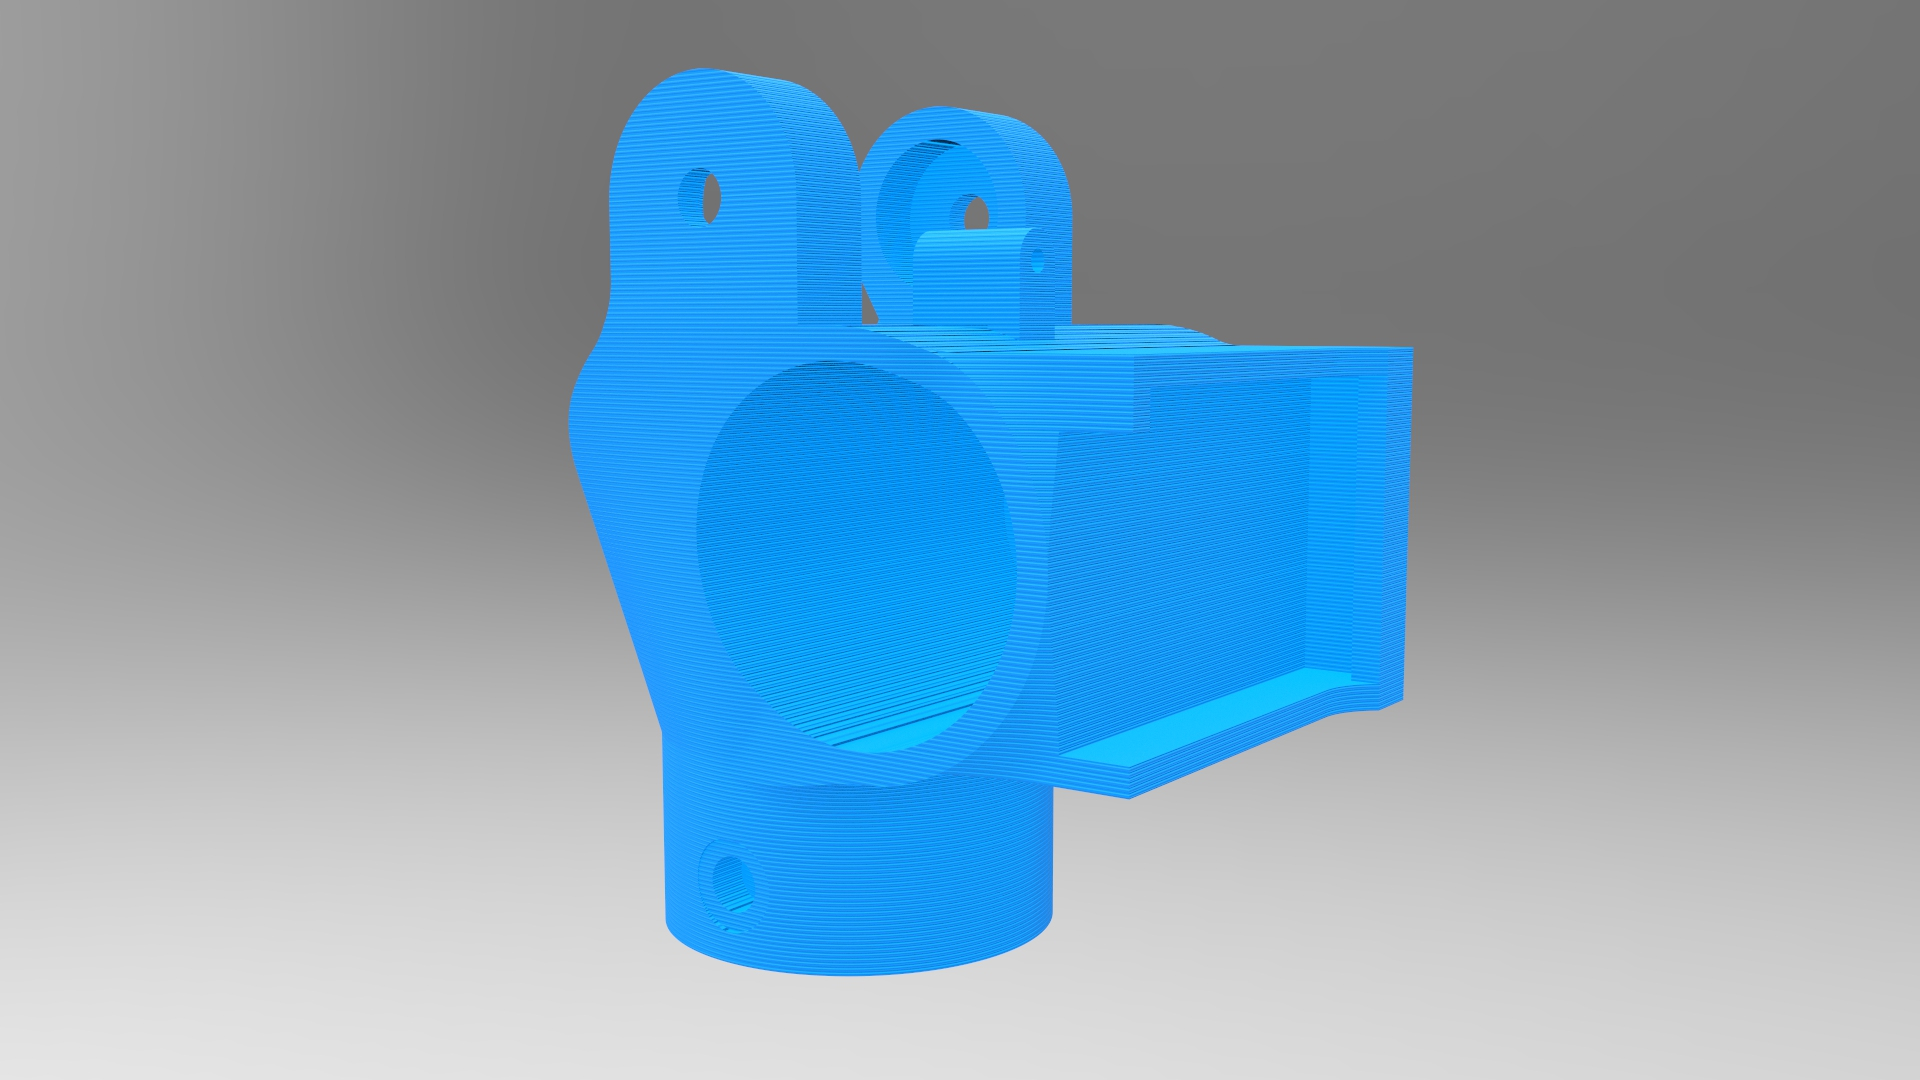
\includegraphics[width=\textwidth]{figures/legs_knee_lower.jpg}
        \caption{Left lower knee}
        \label{fig:lower_knee}
    \end{subfigure}

    \begin{subfigure}[b]{0.49\textwidth}
        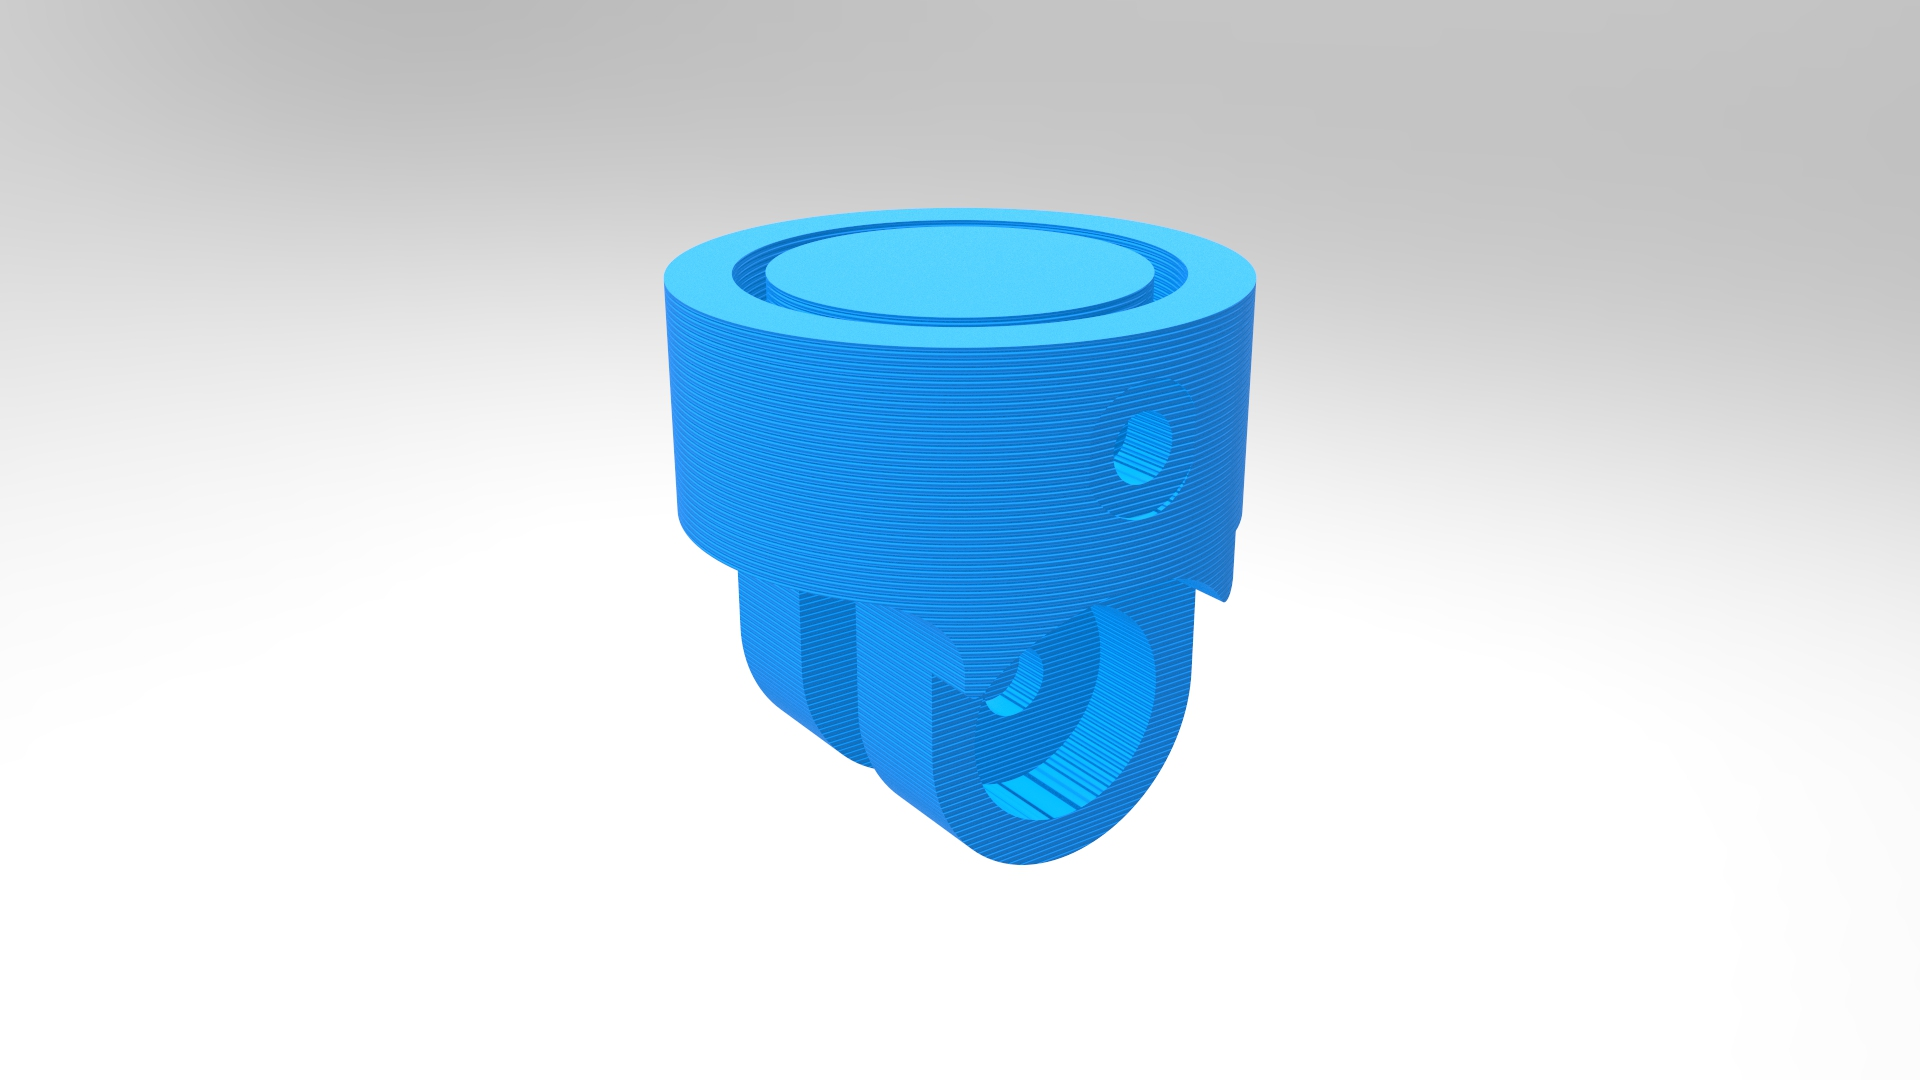
\includegraphics[width=\textwidth]{figures/legs_ankle_upper.jpg}
        \caption{Left upper ankle}
        \label{fig:ankle_upper}
    \end{subfigure}
    \begin{subfigure}[b]{0.49\textwidth}
        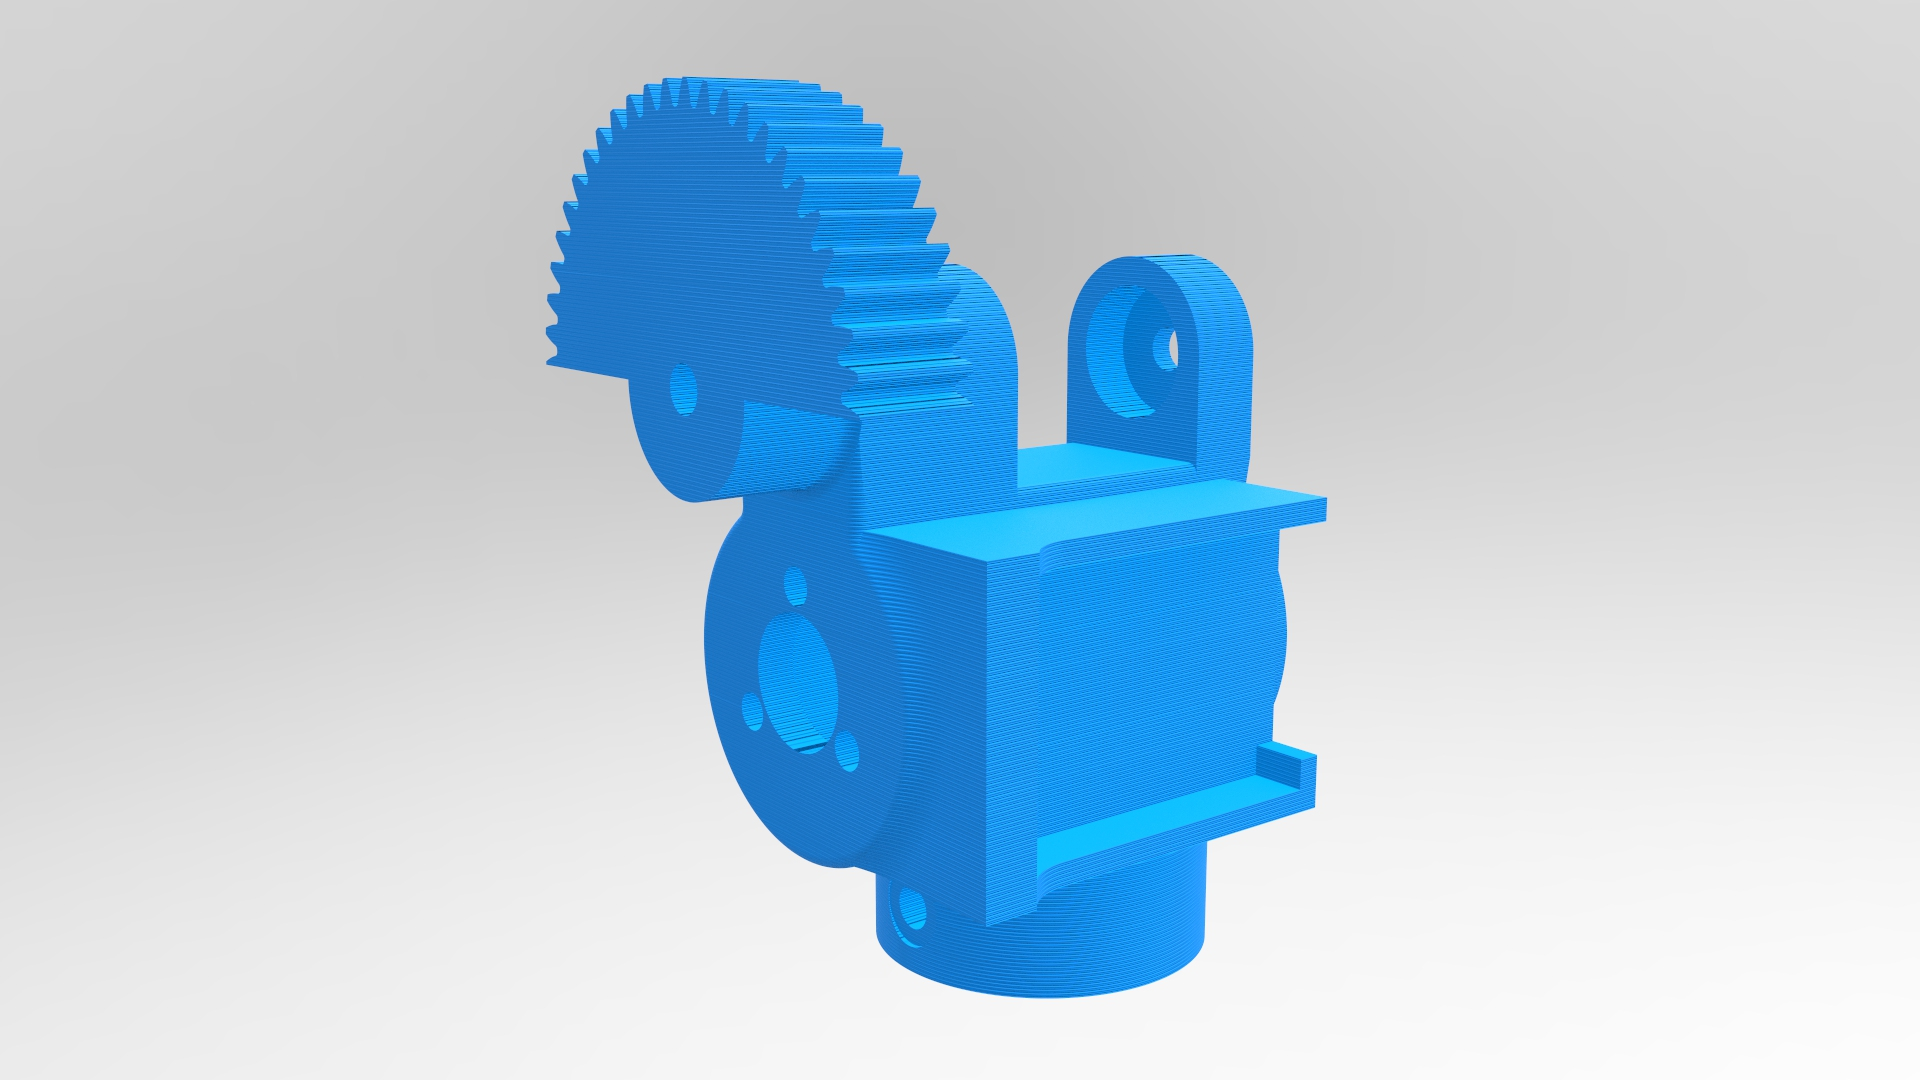
\includegraphics[width=\textwidth]{figures/legs_hip_lower.jpg}
        \caption{Left lower hip}
        \label{fig:hip_lower}
    \end{subfigure}

    \begin{subfigure}[b]{0.49\textwidth}
        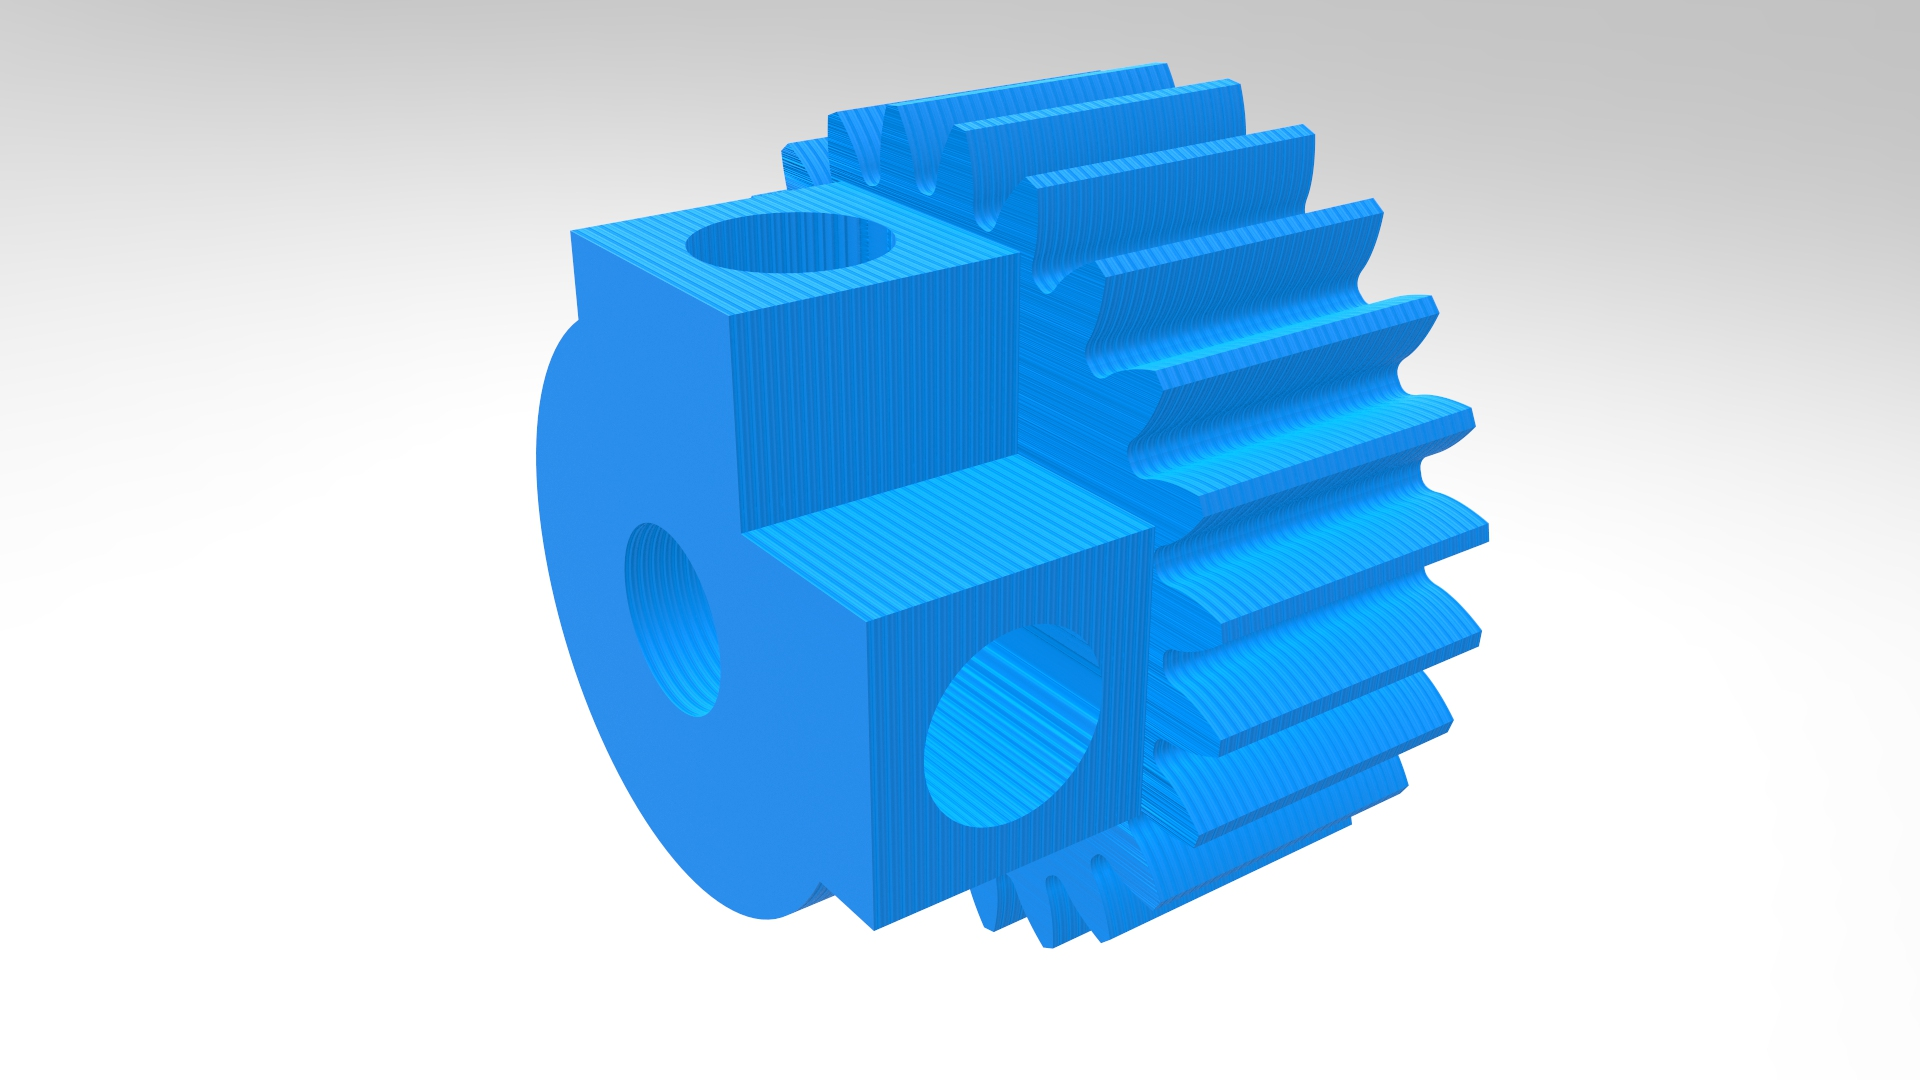
\includegraphics[width=\textwidth]{figures/legs_hip_pinion.jpg}
        \caption{Hip's pinion}
        \label{fig:hip_pinion}
    \end{subfigure}
    \begin{subfigure}[b]{0.49\textwidth}
        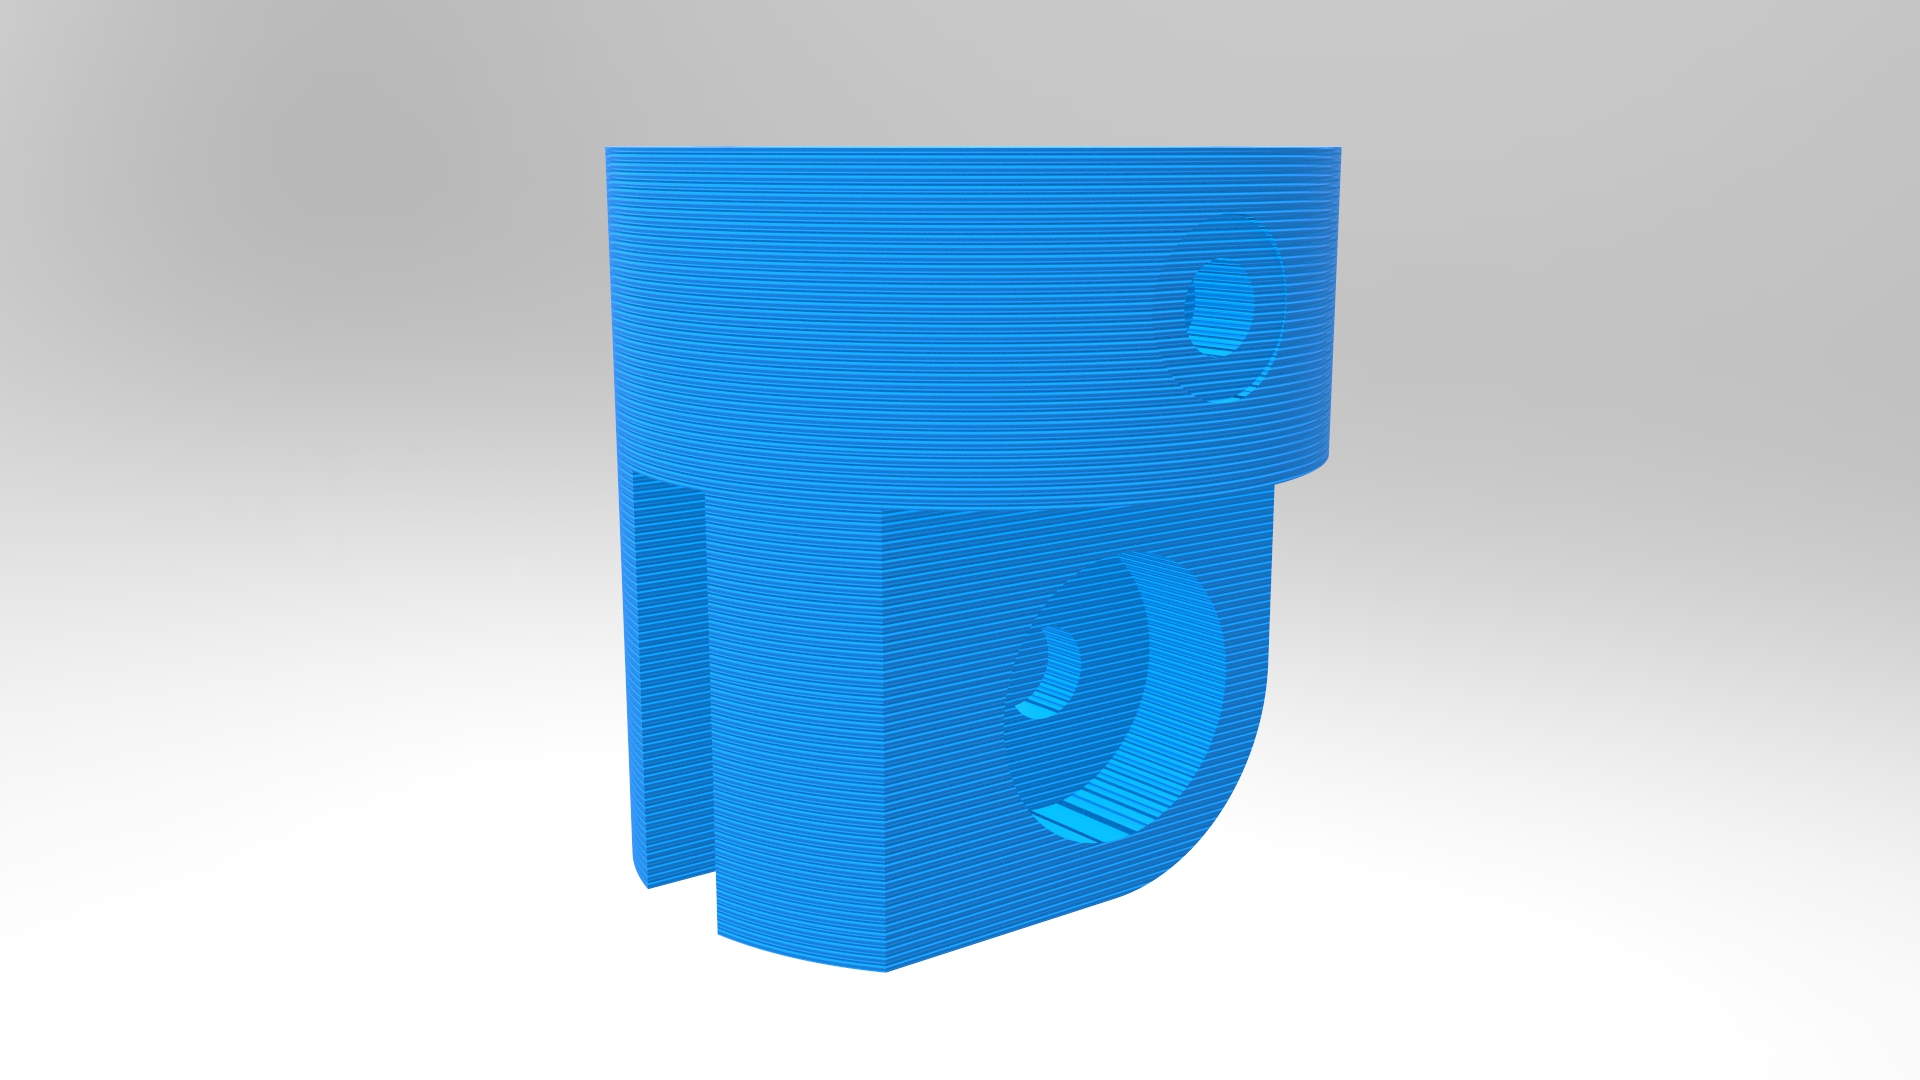
\includegraphics[width=\textwidth]{figures/legs_knee_upper.jpg}
        \caption{Left upper knee}
        \label{fig:knee_upper}
    \end{subfigure}
\end{figure}

% subsection computer_aided_design (end)
%!TEX root = ../../../../report.tex
\subsection{Mechanical limits} % (fold)
\label{sub:mechanical_limits}
The design includes mechanical limits that are used for two reasons:
\begin{enumerate}
  \item \textbf{Calibration}: used as starting points for the relative encoders.
  \item \textbf{Security}: the mechanical limits do not allow the movement further them, which restrict the movement to a predictible behavior protecting then other parts of the robot.
\end{enumerate}

The Figure \ref{fig:joint_limits_hip} shows how the mechanical limits of the hip (both left and right) are implemented in the upper part, spreading an angle of 90 + 60 = 150 degrees.
The Figure \ref{fig:joint_limits_ankle_upper} shows the upper part of the ankle and how the movement of the foot can be of 60 + 50 = 110 degrees.
The mechanical limits of the knee are got with a combination among the lower and upper part of the knee.
These allow movements of 0 + 120 = 120 degrees as shown in the figures \ref{fig:joint_limits_knee_upper} and \ref{fig:joint_limits_knee_lower}.

\begin{figure}[ht!]
    \centering
    \begin{subfigure}[b]{0.49\textwidth}
        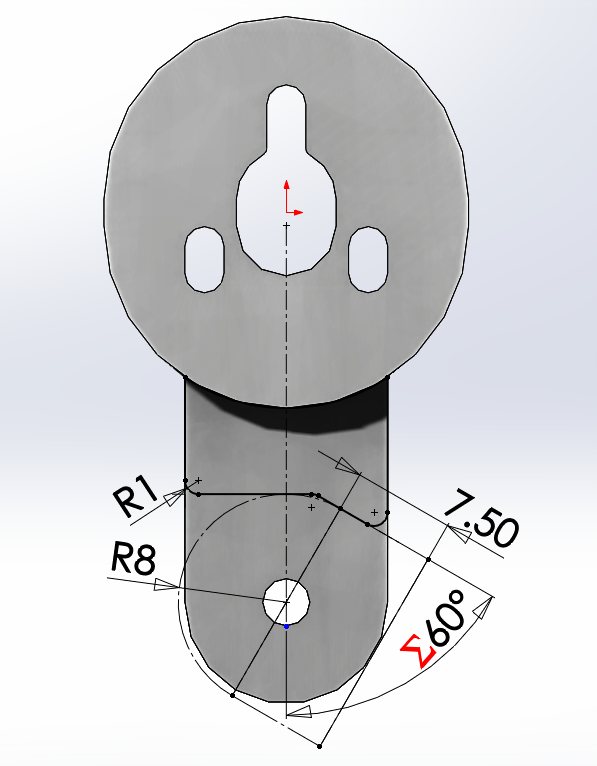
\includegraphics[width=\textwidth]{figures/joint_limits_hip.PNG}
        \caption{Joint limits of the hip}
        \label{fig:joint_limits_hip}
    \end{subfigure}
    \begin{subfigure}[b]{0.49\textwidth}
        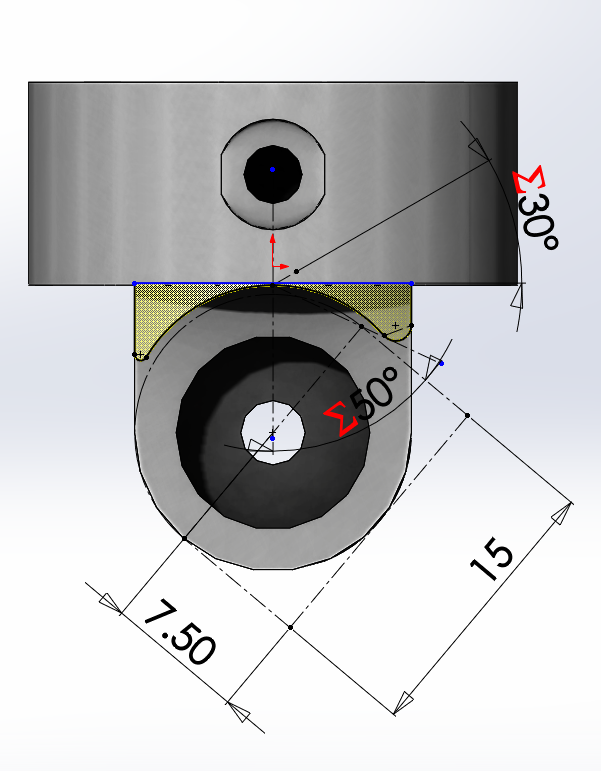
\includegraphics[width=\textwidth]{figures/joint_limits_ankle_upper.PNG}
        \caption{Joint limits of the ankle}
        \label{fig:joint_limits_ankle_upper}
    \end{subfigure}
\end{figure}    

\begin{figure}[ht!]
    \ContinuedFloat % continue from previous page
    \begin{subfigure}[b]{0.49\textwidth}
        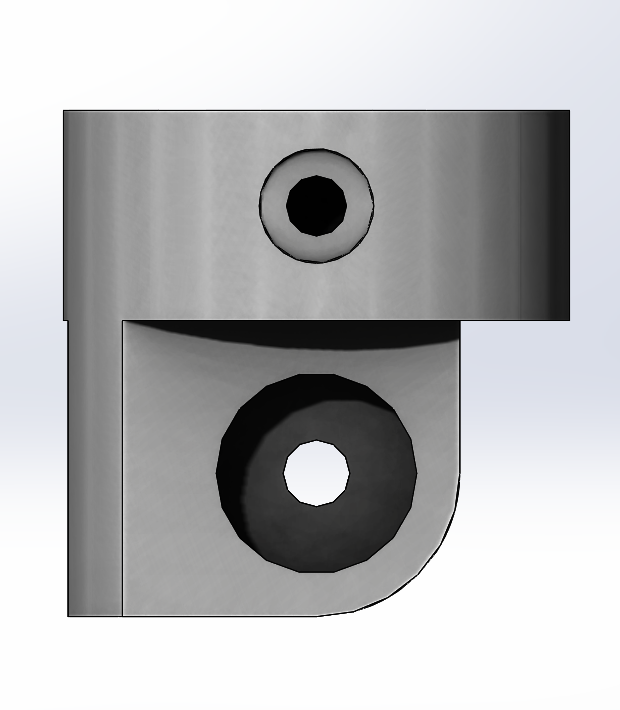
\includegraphics[width=\textwidth]{figures/joint_limits_knee_upper.PNG}
        \caption{Joint limits of the knee: Upper link}
        \label{fig:joint_limits_knee_upper}
    \end{subfigure}
    \begin{subfigure}[b]{0.49\textwidth}
        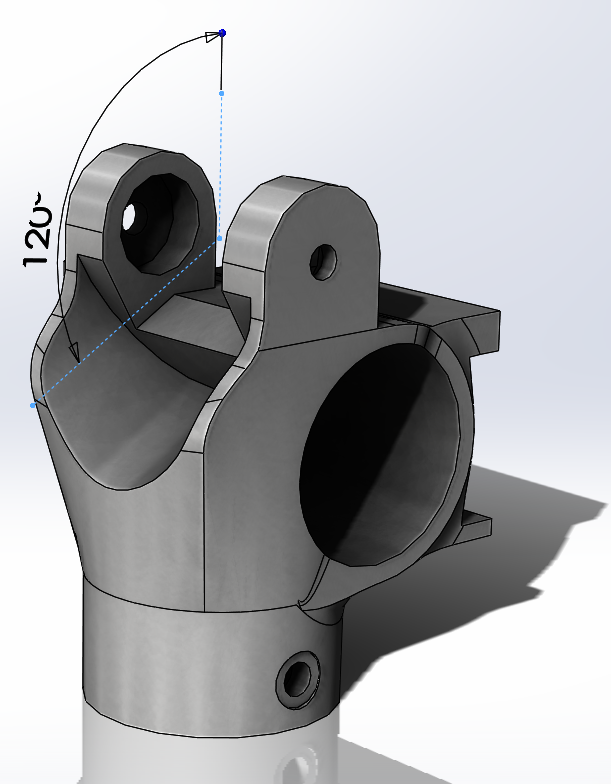
\includegraphics[width=\textwidth]{figures/joint_limits_knee_lower.PNG}
        \caption{Joint limits of the knee: Lower link}
        \label{fig:joint_limits_knee_lower}
    \end{subfigure}
\end{figure}    

% subsection mechanical_limits (end)

% section mechanics (end)